\documentclass[a4paper,12pt]{article}
%\usepackage[latin1]{inputenc}
\usepackage[spanish]{babel}
\usepackage{graphicx}
\usepackage{amsmath}
\usepackage{tcolorbox}% http://ctan.org/pkg/tcolorbox
\usepackage{multicol}
\usepackage{caption}%,subcaption}
\usepackage{jgn}
\spanishdecimal{.}
\usepackage{wrapfig}
\setlength{\textheight}{250mm}
\setlength{\textwidth}{165mm}
\setlength{\topmargin}{-15mm}
\setlength{\oddsidemargin}{0pt}
\pagestyle{empty}


\renewcommand{\labelenumi}{\alph{enumi})}

\begin{document}

\def\imagebox#1#2{\vtop to #1{\null\hbox{#2}\vfill}}
\def\bm#1{{\mbox{\boldmath $#1$}}}
\def\eqdef{\buildrel \rm def \over =}
\def\signo{\mathop{\rm signo}\nolimits}

\definecolor{mycolor}{rgb}{0.122, 0.435, 0.698}% Rule colour
\makeatletter
\newcommand{\mybox}[1]{%
  \setbox0=\hbox{#1}%
  \setlength{\@tempdima}{\dimexpr\wd0+13pt}%
  \begin{tcolorbox}[colframe=mycolor,boxrule=0.5pt,arc=4pt,
      left=6pt,right=6pt,top=6pt,bottom=6pt,boxsep=0pt,width=\@tempdima]
    #1
  \end{tcolorbox}
}
\makeatother



\mbox{}\vspace*{-20mm}

{\centering
{\small\sc %Escuela Técnica Superior de Ingenieros de Caminos, Canales y Puertos (Madrid)}\\*[4mm]
Máster Universitario en Ingeniería de Estructuras, Cimentaciones y Materiales}\\*[4mm]
{\Large\bf Método de los Elementos Finitos 23-24}\\*[4mm]
PRÁCTICAS 4-5: Elasticidad lineal. \\*[4mm]
Ejercicios de repaso \\*[4mm]
}

\section{Ejercicio 1}

En este ejercicio se pide modelizar el ejemplo clásico de la Membrana de Cook, describiéndose su geometría en la Fig.~\ref{figu120} (en mm). La membrana está empotrada en un extremo y sometido a esfuerzo cortante en el opuesto. El esfuerzo aplicado es $F=1.8\ kN$, repartido a lo largo del lado derecho. Las propiedades elásticas del material son $E=70\ GPa$ y $\nu=0.33$, y su espesor es 1 mm. Trabajaremos bajo la hipótesis de tensión plana.
La malla será de tipo estructurada, subdividiendo en 16 partes cada lado del contorno. Se utilizarán el mismo tipo de elemento que en la práctica principal. 
\begin{figure}[!h]
  \begin{center}
    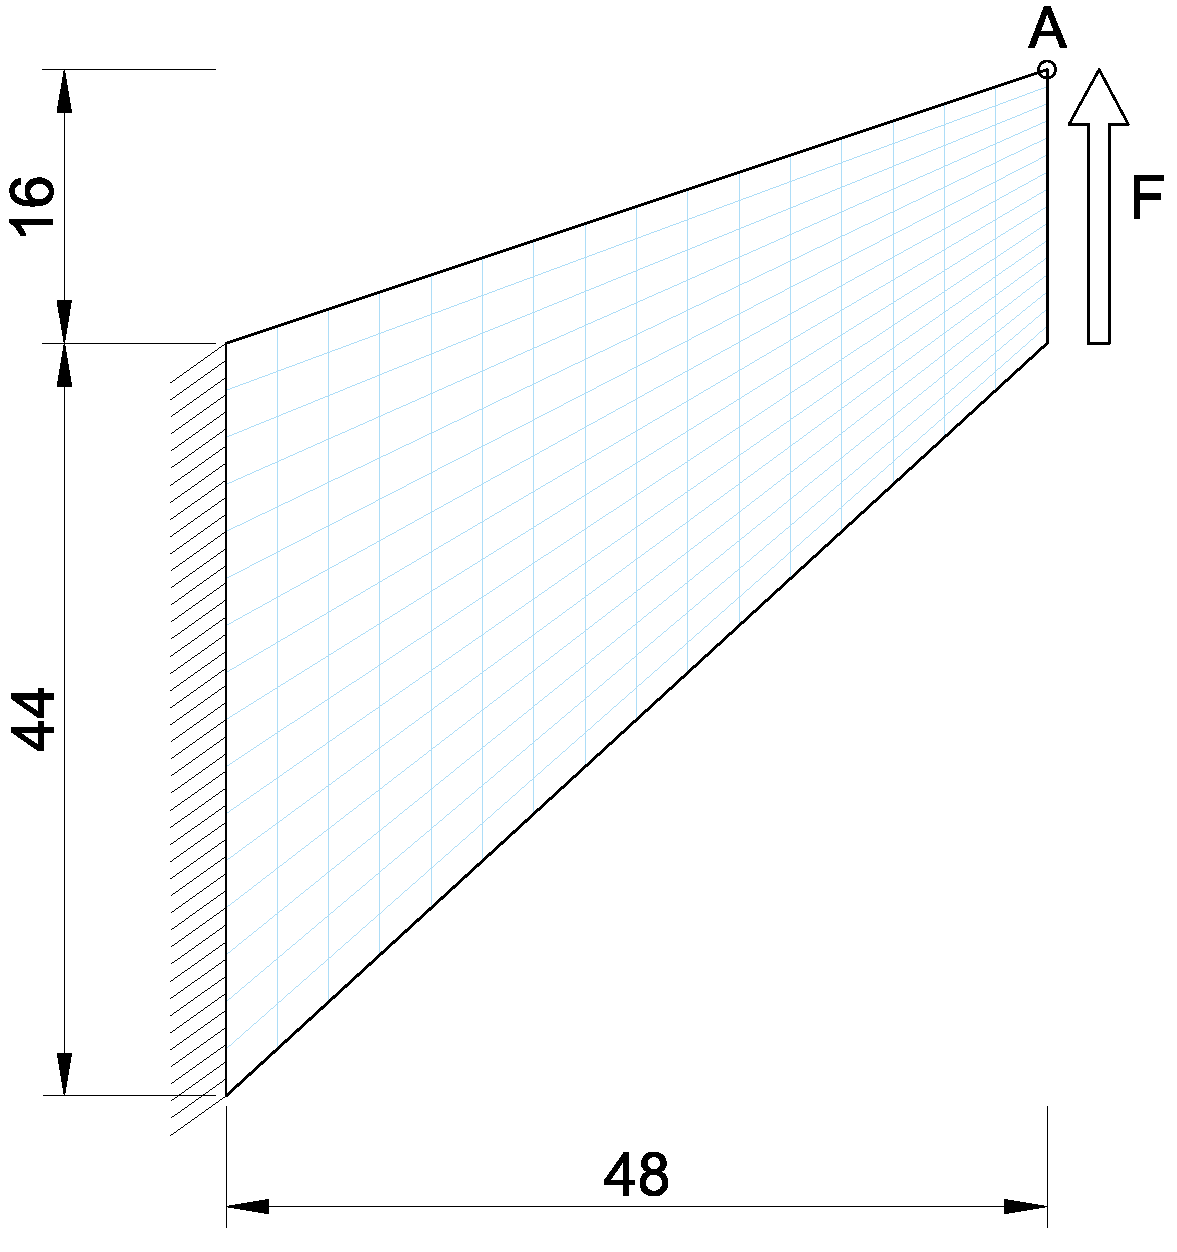
\includegraphics[width=0.45\textwidth]{./figs/membrana1}
  \end{center}
  \caption{Descripción del modelo}
  \label{figu120}
\end{figure}
\begin{enumerate}
\item ¿Cuál es el módulo del desplazamiento del punto A?
  \begin{multicols}{4}
  \mybox{A: 0.807 mm} %ok$
\columnbreak
\mybox{B: 1.125 mm}
\columnbreak
\mybox{C: 0.689 mm}
\columnbreak
\mybox{D: 1.333 mm}
  \end{multicols}
\item El valor máximo de la reacción en el empotramiento es:
  \begin{multicols}{4}
\mybox{A: 1203.0 N}
\columnbreak
\mybox{B: 857.6 N} %ok$
\columnbreak
\mybox{C: 560.3 N}
\columnbreak
\mybox{D: 251.6 N}
  \end{multicols}
\item El valor máximo de la tensión de Von Mises es:
  \begin{multicols}{4}
\mybox{A: 1321.0 MPa}
\columnbreak
\mybox{B: 854.2 MPa} %ok$
\columnbreak
\mybox{C: 1598.3 MPa}
\columnbreak
\mybox{D: 381.6 MPa}
\end{multicols}
\end{enumerate}


\newpage
\section{Ejercicio  2}
A continuación se muestra un ejemplo que formalmente es muy similar al
ejercicio resuelto en la sección anterior. Se trata de una pieza en L
que está empotrada en uno de sus extremos y hay una fuerza repartida
en la mitad de su borde superior. La Fig.~\ref{figu115} resume el
ejemplo.

\begin{figure}[!h]
  \begin{center}
    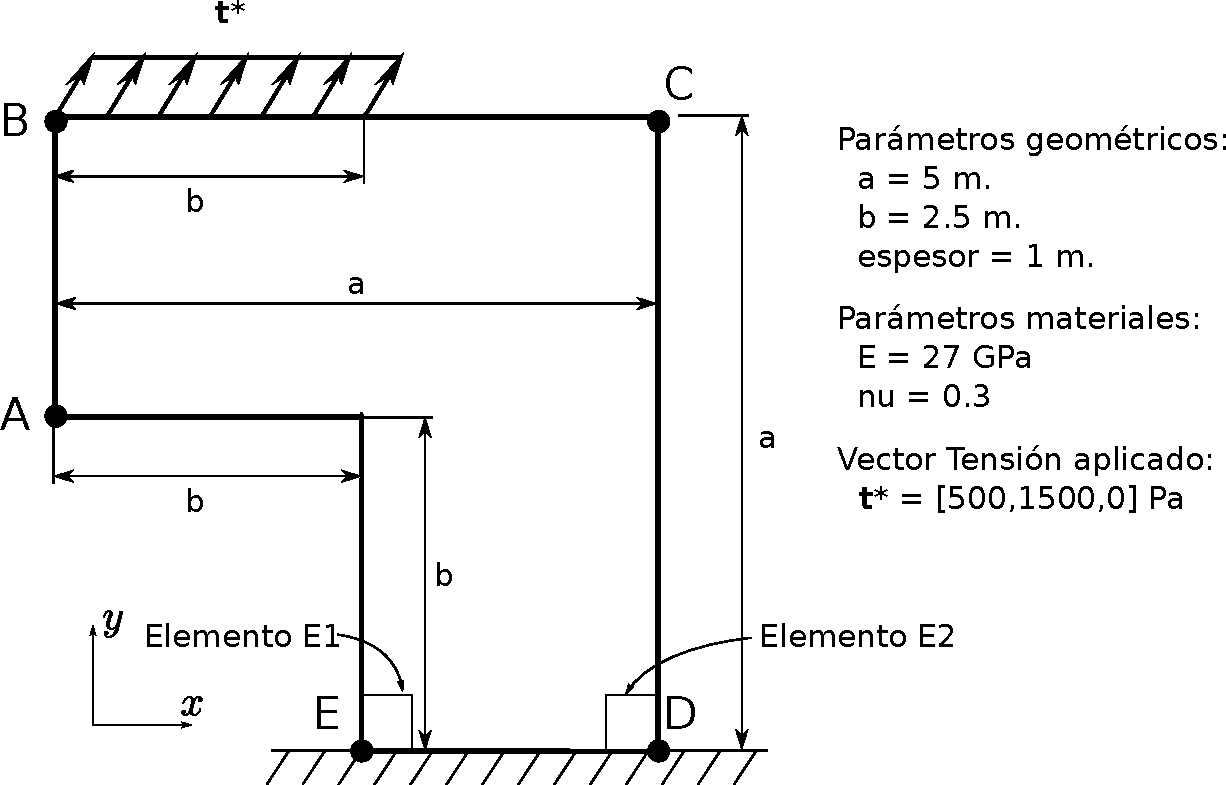
\includegraphics[width=0.65\textwidth]{./figs/imagen115}
  \end{center}
  \caption{Descripción del modelo}
  \label{figu115}
\end{figure}

Para este modelo utilizamos el tipo de elemento cuadrilátero lineal y un tamaño global
de elemento de valor $0.3$ metros, responde las siguientes preguntas:


\begin{enumerate}
\item ¿Cuál es el desplazamiento vertical del punto B?
\begin{multicols}{4}
\mybox{A: 2.821 $\cdot$ 10$^{-6}$ m.}
\columnbreak
\mybox{B: 6.024 $\cdot$ 10$^{-6}$ m.} %OK
\columnbreak
\mybox{C: 2.123 $\cdot$ 10$^{-5}$ m.}
\columnbreak
\mybox{D: 3.254 $\cdot$ 10$^{-9}$ m.}
\end{multicols}
\item ¿Cul es el desplazamiento horizontal del punto C?
\begin{multicols}{4}
\mybox{A: 1.627 $\cdot$ 10$^{-6}$ m.}
\columnbreak
\mybox{B: 4.741 $\cdot$ 10$^{-6}$ m.} %OK
\columnbreak
\mybox{C: 2.321 $\cdot$ 10$^{-5}$ m.}
\columnbreak
\mybox{D: 5.237 $\cdot$ 10$^{-9}$ m.}
\end{multicols}
\item ¿Cuál es la componente $\sigma_{22}$ del tensor de tensiones en el 
centroide del elemento $E1$?
\begin{multicols}{4}
\mybox{A: 1782 Pa.}
\columnbreak
\mybox{B: 17413 Pa.}
\columnbreak
\mybox{C: 7174 Pa.}
\columnbreak
\mybox{D: 14904 Pa.} %OK
\end{multicols}
\item ¿Cuál es el valor máximo (en valor absoluto) de la tensión principal
mínima $\sigma_3$ en el camino $EC$?
\begin{multicols}{4}
\mybox{A: -851 Pa.}
\columnbreak
\mybox{B: -8801 Pa.}
\columnbreak
\mybox{C: -1984 Pa.}
\columnbreak
\mybox{D: -3366 Pa.}%OK
\end{multicols}
\end{enumerate}
%\hspace{20mm}\hrulefill$\star$\hrulefill\hspace{20mm}

\newpage

\section{Ejercicio  3}

Queremos estudiar el comportamiento mecánico del modelo presentado en la Fig.~\ref{figu116}, donde los segmentos circulares tienen un radio igual a 1 m. La pieza tiene un estado de \textit{tensión plana} con las siguientes condiciones de contorno:
\begin{itemize}
\item Todos los desplazamientos son nulos en el segmento $AB$.
\item En el segmento $EF$ imponemos el valor del desplazamiento $u_x^*=0.01$ m.
\item Hay una fuerza vertical concentrada de valor $F_y=200$ N.
\end{itemize}

El comportamiento material es elástico lineal e isótropo con módulos elásticos  $E=1000000$ Pa.~y $\nu=0.25$. Para construir el problema discreto usamos una malla con los siguientes parámetros: \textit{quad-dominated, quadratic y con un tamaño global de 0.9}.

\begin{figure}[!h]
  \begin{center}
    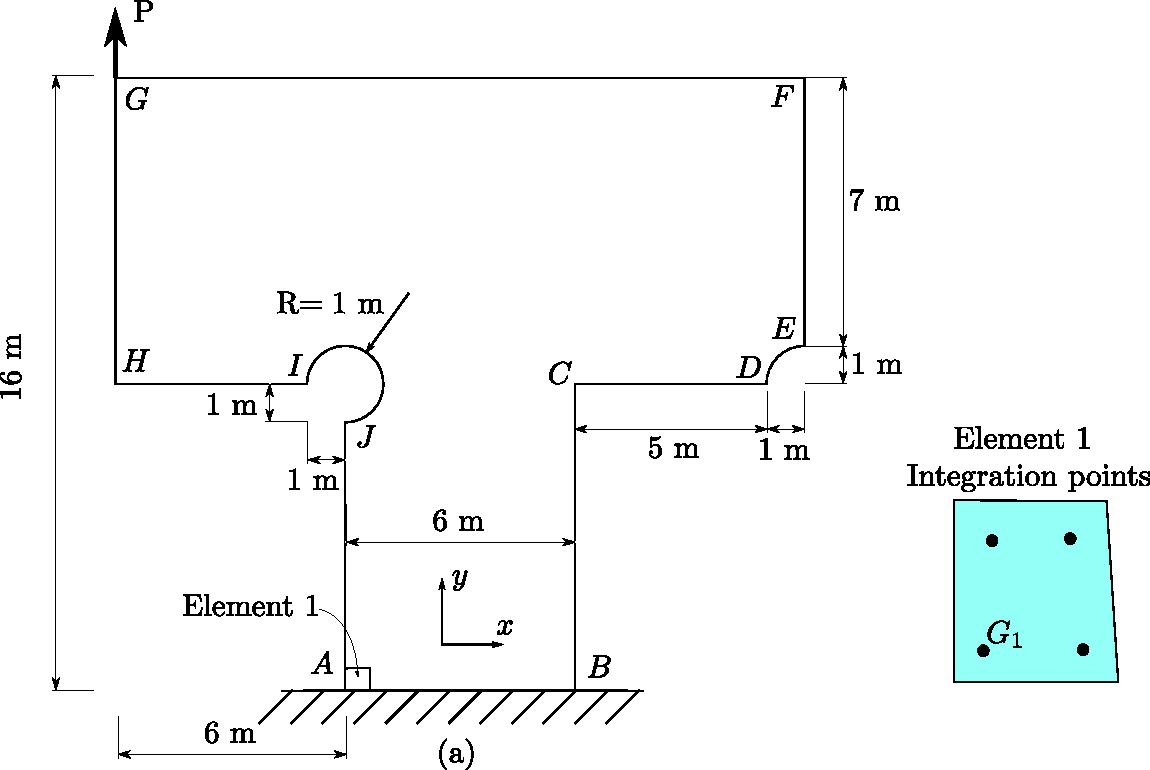
\includegraphics[width=0.65\textwidth]{./figs/imagen116}
  \end{center}
  \caption{Descriptión del modelo}
  \label{figu116}
\end{figure}

Para este modelo responde las siguientes preguntas:



\begin{enumerate}
\item Cuál es el desplazamiento vertical del punto H?
  \begin{multicols}{4}
  \mybox{A: 0.0094 m.} %ok$
\columnbreak
\mybox{B: 0.0025 m.}
\columnbreak
\mybox{C: 0.0125 m.}
\columnbreak
\mybox{D: 0.0003 m.}
  \end{multicols}
\item Cuál es el desplazamiento horizontal del punto J?
  \begin{multicols}{4}
\mybox{A: 0.0012 m.}
\columnbreak
\mybox{B: 0.0050 m.} %ok$
\columnbreak
\mybox{C: 0.0006 m.}
\columnbreak
\mybox{D: 0.0181 m.}
  \end{multicols}
\item Cuál es la componente $\sigma_{22}$ del tensor de tensiones en el punto de integración $G_1$ del elemento 1 (ver figura)?
  \begin{multicols}{4}
  \mybox{A: 710 Pa.} %ok$
\columnbreak
\mybox{B: 1412 Pa.}
\columnbreak
\mybox{C: 172 Pa.}
\columnbreak
\mybox{D: 904 Pa.}
  \end{multicols}
\item Cuál es el valor máximo de la tensión principal máxima en el camino $AF$?
  \begin{multicols}{4}
   \mybox{A: 51 Pa.}
\columnbreak
\mybox{B: 894 Pa.} %ok$
\columnbreak
\mybox{C: 1384 Pa.}
\columnbreak
\mybox{D: 323 Pa.}
\end{multicols}
\item Cuál es la suma de las fuerzas de reacción horizontales en la base $AB$?
  \begin{multicols}{4}
   \mybox{A: -231.75 N.}%ok
\columnbreak
\mybox{B: -124.87 N.}
\columnbreak
\mybox{C: -13 N.}
\columnbreak
\mybox{D: -323 N.}
  \end{multicols}
\end{enumerate}
%\hspace{20mm}\hrulefill$\star$\hrulefill\hspace{20mm}


\vspace{10mm}

\section{Ejercicio 4}
El puente de la Fig.~\ref{figuprop1}, de ancho 3,5 m, se encuentra empotrado en pilas y estribos en las áreas verticales de contacto con el terreno circundante. El módulo de Young del material es de 30.0 GPa, el coeficiente de Poisson es $\nu=0.2$ y el peso específico es $\gamma=24000 \mathrm{~N} / \mathrm{m}^{3}$. Las acciones a considerar serán el peso propio y el efecto de un sismo que se supondrá equivalente a una fuerza volumétrica, distribuida transversalmente al puente, de valor $1000 \mathrm{~N} / \mathrm{m}^{3}$, actuando en el sentido AB (Fig.~\ref{figuprop1}).

Se desea estudiar el comportamiento estructural de este puente ante las dos acciones mencionadas. Teniendo en cuenta las simetrías del problema, se preparará un modelo con Abaqus de la mitad del puente tal y como se indica en la Fig.~\ref{figuprop1}, donde se detalla la geometría de la estructura.

\begin{figure}[!h]
  \begin{center}
    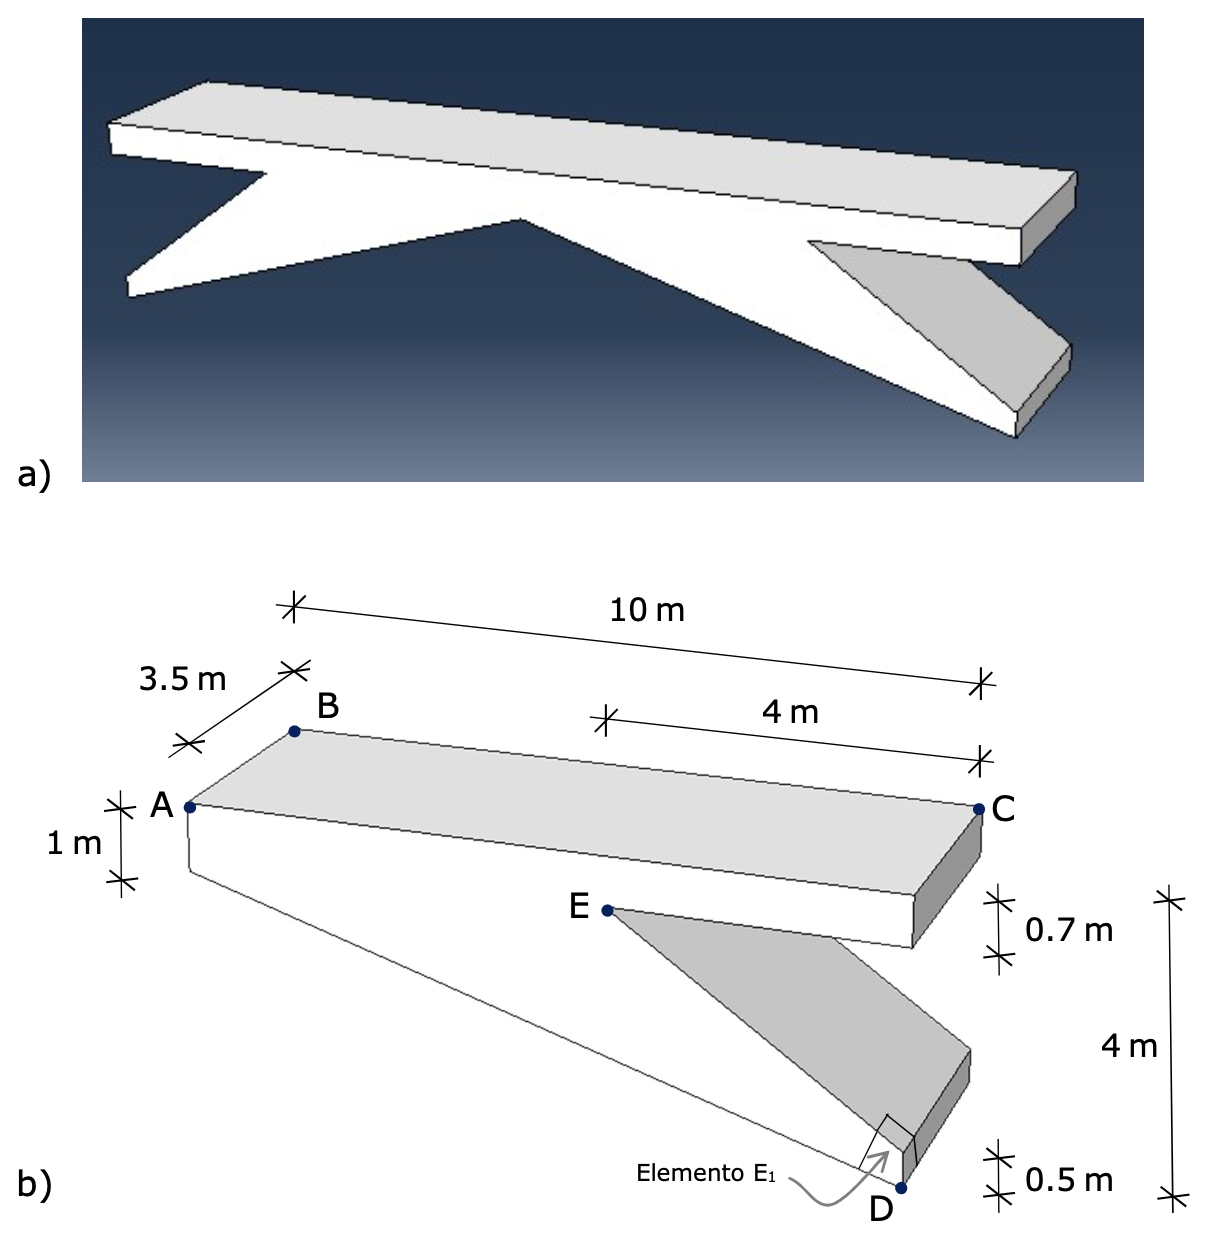
\includegraphics[width=0.45\textwidth]{./figs/prop}
  \end{center}
  \caption{Descripción del ejercicio propuesto}
  \label{figuprop1}
\end{figure}

Responde las preguntas que vienen a continuación teniendo en cuenta que el elemento a emplear será el hexaedro de 8 nodos con integración reducida C3D8R y el tamaño del elemento a utilizar en el mallador de Abaqus será $0.55 \mathrm{~m}$.

\begin{enumerate}
\item Flecha vertical (valor absoluto) en el punto B:
  \begin{multicols}{4}
  \mybox{A: $3.1\cdot 10^{-5}$ $m$} 
\columnbreak
\mybox{B: $42.1\cdot 10^{-3}$ $m$}
\columnbreak
\mybox{C: $42.1\cdot 10^{-5}$ $m$} %ok$
\columnbreak
\mybox{D: $3.1\cdot 10^{-3}$ $m$}
  \end{multicols}

\item M\'axima tensi\'on de tracci\'on en el modelo:
  \begin{multicols}{4}
\mybox{A:  $0.09$ MPa}
\columnbreak
\mybox{B: $-1.642$ MPa} 
\columnbreak
\mybox{C: $0.393$ MPa}%ok$
\columnbreak
\mybox{D: $450.6$ MPa}
\end{multicols}

\item M\'inima tensi\'on de compresi\'on en el centroide del elemento E1:
  \begin{multicols}{4}
\mybox{A:   $-0.113$ MPa}
\columnbreak
\mybox{B: $0.5$ MPa} 
\columnbreak
\mybox{C: $-1.47$ MPa}%ok$
\columnbreak
\mybox{D:  $0.113$ MPa}
\end{multicols}
\item Tensi\'on vertical en el punto D:
  \begin{multicols}{4}
\mybox{A:  $-283.5$ kPa}%ok$
\columnbreak
\mybox{B:  $-3048.4$ kPa} 
\columnbreak
\mybox{C:  $-30.9$ kPa}
\columnbreak
\mybox{D:   $117.9$ kPa}
\end{multicols}
\end{enumerate}

\clearpage
\section{Ejercicio 5}

Se desea estudiar el comprtamiento de una esfera de radio interior $2\,\text{m}$ y radio exterior $3\,\text{m}$ sometida a una presión uniforme interior de $10^{4}\,\text{Pa}$. 
El módulo de Young del material es $30\cdot10^{9}\,\text{Pa}$ y  el coeficiente de Poisson $\nu=0.2$. No se 
considerará el peso propio.

Para obtener los resultados se analizará un modelo formado por un octavo de la esfera teniendo en cuenta las
simetrías del problema.

El elemento a usar será el elemento hexaedro de 8 nodos con integración reducida C3D8R y el tamaño de elemento a utilizar 
en el mallador de abaqus será $0.3\, \text{m}$.
Para el mallado se utilizará el mallado de tipo estructurado con hexaedros.


\begin{center}
	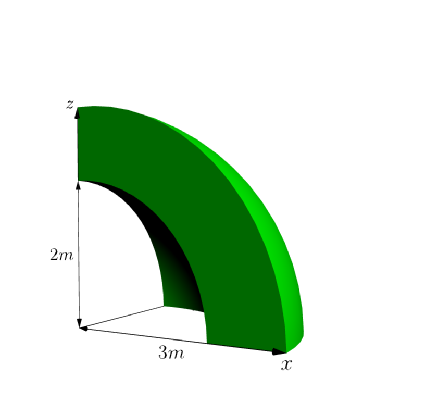
\includegraphics[width=0.5\textwidth]{figs/deposito_esfer.pdf}
\end{center}
\vspace{1.5mm}

%%%%%%%%%%%%%%%%%%%%%%%%%%%%%%%%%%%%%%%%%%%%%%%%%%%%%%%%%%%%%%%%%%%%%%%%%%%%%
\begin{enumerate}
\item Incremento del radio interior de la esfera.
  \begin{multicols}{4}
  \mybox{A: $7.03\cdot 10^{-7}$ m} %ok
\columnbreak
\mybox{B: $1.09\cdot 10^{-6}$ m}
\columnbreak
\mybox{C: $3.28\cdot 10^{-5}$ m}
\columnbreak
\mybox{D: $9.82\cdot 10^{-5}$ m}
  \end{multicols}

%%%%%%%%%%%%%%%%%%%%%%%%%%%%%%%%%%%%%%%%%%%%%%%%%%%%%%%%%%%%%%%%%%%%%%%%%%%%
\item Máxima tensión de tracción del modelo.
\begin{multicols}{4}
  \mybox{A: $4.89\cdot 10^{3}$ Pa}
\columnbreak
\mybox{B: $2.21\cdot 10^{5}$ Pa}
\columnbreak
\mybox{C: $1.01\cdot 10^4$ Pa} %ok
\columnbreak
\mybox{D: $6.43\cdot 10^{5}$ Pa}
  \end{multicols}
%%%%%%%%%%%%%%%%%%%%%%%%%%%%%%%%%%%%%%%%%%%%%%%%%%%%%%%%%%%%%%%%%%%%%%%%%%%%
\item Cambio de espesor de la esfera (en valor absoluto).
\begin{multicols}{4}
  \mybox{A: $8.81\cdot 10^{-7}$ m}
\columnbreak
\mybox{B: $2.27\cdot 10^{-7}$ m} %ok
\columnbreak
\mybox{C:$4.18\cdot 10^{-6}$ m}
\columnbreak
\mybox{D: $2.17\cdot 10^{-6}$ m}
  \end{multicols}
%%%%%%%%%%%%%%%%%%%%%%%%%%%%%%%%%%%%%%%%%%%%%%%%%%%%%%%%%%%%%%%%%%%%%%%%%%%%%%

%%%%%%%%%%%%%%%%%%%%%%%%%%%%%%%%%%%%%%%%%%%%%%%%%%%%%%%%%%%%%%%%%%%%%%%%%%%%%%
\item Máxima tensión de Von Mises.
\begin{multicols}{4}
  \mybox{A: $8.25\cdot 10^{3}$ Pa}
\columnbreak
\mybox{B:$3.98\cdot 10^{5}$ Pa}
\columnbreak
\mybox{C:$6.15\cdot 10^{4}$ Pa}
\columnbreak
\mybox{D: $1.76\cdot 10^4$ Pa} %ok
  \end{multicols}

\end{enumerate}


%\section{Ejercicio propuesto 3}
%\label{sec:probprop2}
%
%Una estructura está formada por un cilindro macizo de radio interior $21.5\,\text{m}$, radio exterior $27.5\,\text{m}$, eje vertical 
%y altura $h=21.5\,\text{m}$. Este cilindro se encuentra empotrado en la base. Sobre el cilindro y unida a él, se encuentra
%una cúpula tambien maciza que deja una abertura superior de diámetro $9m$. Tanto la superficie 
%interior de la cúpula como la exterior se unen con tangente común con el cilindro. El radio interior de la 
%cúpula es $21.5\,\text{m}$ estando situado el centro en el eje del cilindro y la superficie exterior de 
%la cúpula se obtiene como la revolución de un arco de radio $22.53\,\text{m}$ alrededor del eje vertical del cilindro y que tiene 
%su centro en el plano del arco situado a una distancia $4.97\,\text{m}$ del eje.
%El módulo de Young del material es $2\cdot10^{10}\,\text{Pa}$, el coeficiente de Poisson es $\nu=0.25$ y el peso específico 
%del material es $\gamma=25000\,\text{N/m}^{3}$.
%
%Se desea estudiar el comportamiento de esta estructura ante el peso propio de la misma para lo que se deberá preparar
%un modelo con abaqus de un cuarto de la misma teniendo en cuenta las simetrías del problema.
%
%El elemento a usar será el elemento hexaedro de 8 nodos con integración reducida C3D8R y el tamaño de elemento a utilizar 
%en el mallador de abaqus será $3. \text{m}$.
%
%
%\begin{center}
%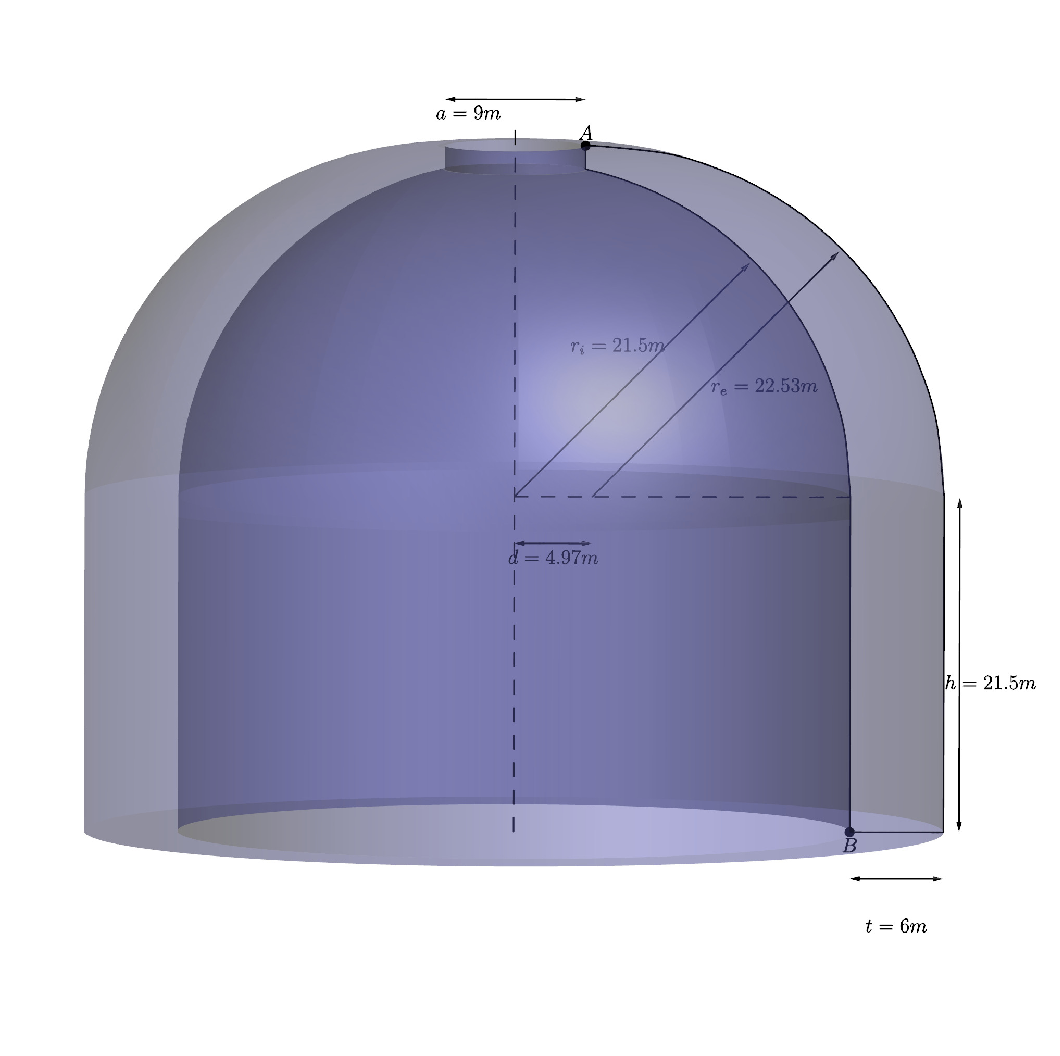
\includegraphics[width=0.8\textwidth]{panteon3.pdf}
%\end{center}
%
%\subsection{Resultados}
%
%\begin{itemize}
%\item Flecha vertical (positivo hacia abajo) en el punto más alto (punto $A$ de la figura).
%     $0.0021$ m
%\item Tensión vertical en la base en el punto más cercano al eje (punto $B$ de la figura).
%    $-829419$ Pa
%\item Tensión circunferencial en la parte más alta del modelo.
%    $-693099$ Pa
%\item Tensión media cortante (en dirección radial) en la superficie de unión del cilindro con la cúpula.
%    $35000$ Pa
%\item Máxima tensión de compresión (siendo la compresión negativa) en el modelo.
%    $-1.10\cdot 10^6$ Pa
%\end{itemize}

\clearpage
\section{Ejercicio 6}
\label{sec:probprop3}


Un puente está formado por un tablero de espesor $2\,\text{m}$, ancho $10\,\text{m}$, un arco de medio punto central de radio $20\,\text{m}$, y dos 
medios arcos de medio punto laterales del mismo radio. El puente está empotrado en las dos bases indicadas en 
la figura de ancho $3\,\text{m}$ y también está empotrado en los estribos. 
El módulo de Young del material es $2\cdot10^{10} \text{Pa}$, el coeficiente de Poisson es $\nu=0.25$ y el peso específico 
del material es $\gamma=25000\, \text{N/m}^{3}$.

Se desea estudiar el comportamiento de este puente ante el peso propio del mismo para lo que se deberá preparar
un modelo con abaqus de un cuarto del mismo teniendo en cuenta las simetrías del problema.

El elemento a usar será el elemento hexaedro de 8 nodos con integración reducida C3D8R y el tamaño de elemento a utilizar 
en el mallador de abaqus será $1.2\,\text{m}$.

\begin{center}
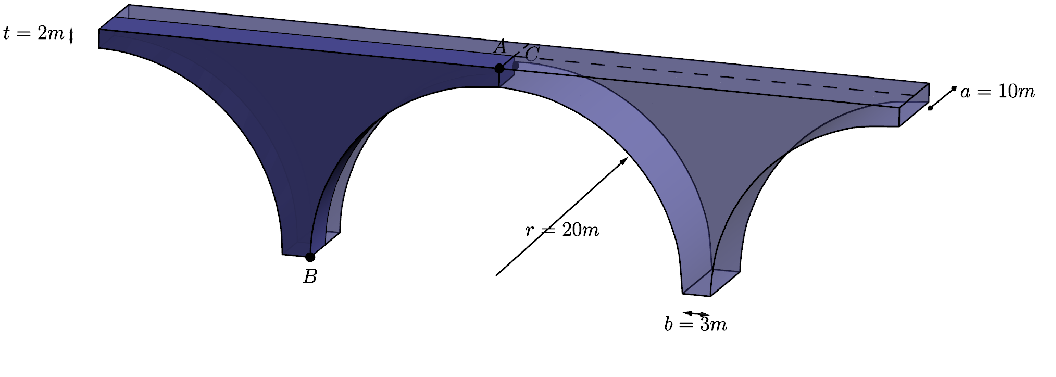
\includegraphics[width=1.0\textwidth]{puente2.pdf}
\end{center}

\subsection{Resultados}

\begin{itemize}
	\item Flecha vertical (positivo hacia abajo) en la superficie del tablero en un borde de la sección central del puente, 
 punto $A$ de la figura.
    {\tt $0.0032$ m}
\item Tensión de compresión vertical en el arranque del arco central (medida en el punto correspondiente a la superficie frontal 
del puente, punto $B$ de la figura).
    {$-2.173\cdot 10^6$ Pa}
\item Tensión longitudinal media en la superficie de la sección central del tablero.
    {$-922440$ Pa}
\item Tensión cortante vertical en el centro de la sección central del tablero (punto $C$ de la figura).
    {$-13391$ Pa}
\item  Máxima tensión de compresión (siendo la compresión negativa) en el modelo.
    {$-3.241\cdot 10^6$ Pa}
\end{itemize}

\clearpage
\section{Ejercicio 7}
\label{sec:probprop4}


Un puente está formado por múltiples pilas de altura $12\,\text{m}$ unidas entre sí mediante un tablero de canto variable. El espesor mínimo del tablero es $1.5\,\text{m}$ y el 
ancho del puente es de $7\,\text{m}$. Para un estudio simplificado del efecto de un sismo sobre el puente se va a hacer
un análisis considerando una pila y parte del tablero de forma simétrica. 
Las acciones a considerar van a ser el peso propio y una fuerza volumétrica distribuida en el sentido 
transversal del puente de valor $1000\,\text{N/m}^{3}$ actuando en el sentido de $A$ a $D$.
El puente está empotrado en las bases de las pilas. 
El módulo de Young del material es $30\,\text{GPa}$, el coeficiente de Poisson es $\nu=0.2$ y el peso específico 
del material es $\gamma=25000\,\text{N/m}^{3}$.

Se desea estudiar el comportamiento de este puente ante la combinación de las dos cargas
mediante un modelo con abaqus que represente un módulo del mismo, tal como se refleja en la figura,  teniendo en cuenta las simetrías del problema.

El elemento a usar será el elemento hexaedro de 8 nodos con integración reducida C3D8R y el tamaño de elemento a utilizar 
en el mallador de abaqus será $1.\,\text{m}$.


\begin{center}
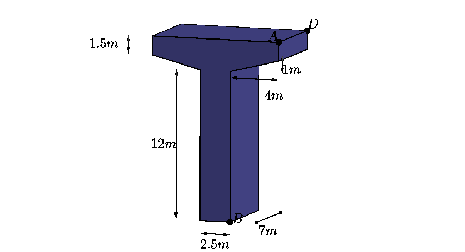
\includegraphics[width=1.2\textwidth]{puente3.pdf}
\end{center}


\subsection{Resultados}

\begin{itemize}
	\item Flecha vertical (positivo hacia abajo) en la superficie del tablero en el punto $A$
de la figura.
    {\tt $0.000174$ m}
\item Flecha vertical (positivo hacia abajo) en la superficie del tablero en el punto $D$
de la figura.
    {\tt $0.000238$ m}
\item Tensión de compresión vertical en la base de la pila 
del puente, punto $B$ de la figura).
    {$-3.907\cdot 10^5$ Pa}
\item Tensión de Von Mises en la base de la pila 
del puente, punto $B$ de la figura).
    {$3.607\cdot 10^5$ Pa}
\item Movimiento horizontal del tablero (en valor absoluto) en la dirección transversal medido en el punto $D$ de la figura.
    {$0.000114\,$ m}
\item Cual es movimiento horizontal del tablero (en valor absoluto) en la dirección transversal medido en el punto $A$ de 
la figura.
    {$0.000109\,$ m}
\item Cual es la máxima tensión de tracción en el modelo.
    {$1.81\cdot 10^5$ Pa}
\item Máxima tensión de compresión en el modelo.
	{$-7.025\cdot 10^5$ Pa}
\end{itemize}


%%%%%%%%%%%%%%%%%%%%%%%%%%%%%%%%%%%%%%%%%%%%%%%%%%%%%%%%%%%%%%%%%%%%%%%%%%%%%%
\clearpage
\section{Ejercicio 8}
\label{sec:probprop5}

Un dique de hormigón tiene sección de trapecio simétrico. El ancho en 
la base es de  $16\,\text{m}$, el ancho en la coronación $4\,\text{m}$ y 
la altura del dique es de $6\,\text{m}$. La longitud del dique es de $30\,\text{m}$.
Se va a hacer un estudio simplificado del efecto de un sismo sobre el dique.
Las acciones a considerar van a ser el peso propio, una sobrecarga en la coronación, otra sobrecarga en uno de los taludes  y una fuerza volumétrica distribuida actúando en el
sentido de $A$ a $B$ (Ver figura).
El valor de la sobrecarga en la coronación es de $3000\,\text{Pa}$, la sobrecarga (vertical) en
el talud $BEFC$ es de  $10000\,\text{Pa}$ y  la fuerza volumétrica transversal es
  $2000\,\text{N/m}^{3}$ actuando en el sentido de $A$ a $B$.
El módulo de Young del material es $30\,\text{GPa}$, el coeficiente de Poisson es $\nu=0.2$ y el peso específico
del material es $\gamma=25000\,\text{N/m}^{3}$.
El dique se considera fijo en todas direcciones en la base y en la sección $ABCD$. 

Se desea estudiar el comportamiento del dique ante la combinación de las cargas antedichas
mediante un modelo con abaqus.

El elemento a usar será el elemento hexaedro de 8 nodos con integración reducida C3D8R y el tamaño de elemento a utilizar 
en el mallador de abaqus será $1.8\,\text{m}$.


\begin{center}
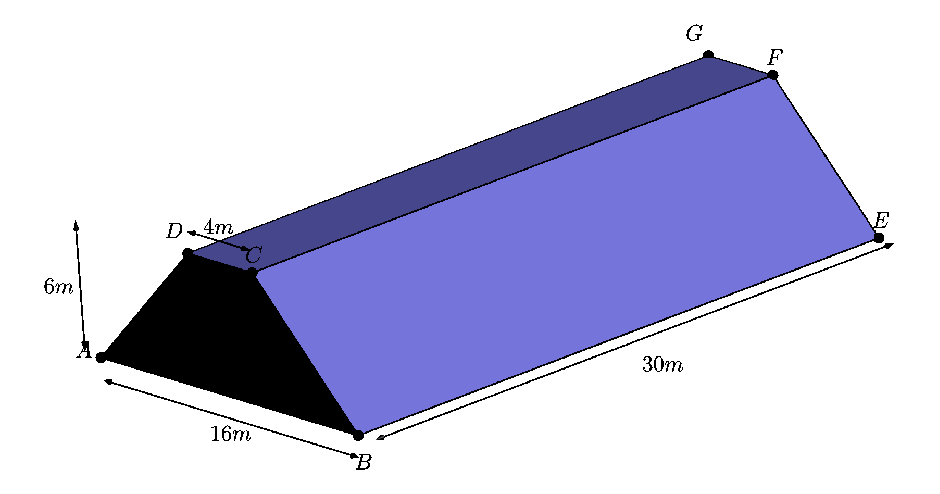
\includegraphics[scale=1.0]{dique.pdf}
\end{center}



\subsection{Resultados}

\begin{itemize}
\item Flecha vertical (positivo hacia abajo) en el punto $F$ de la figura del dique.
    {\tt $1.44\cdot 10^{-5}$ m}
\item Flecha vertical (positivo hacia abajo) en el punto $G$ de la figura del dique.
    {\tt $1.25\cdot 10^{-5}$ m}
\item Tensión de compresión vertical en la base del dique en el  punto $B$ de la figura.
    {$-2.98\cdot 10^4$ Pa}
\item Tensión de compresión vertical en la base del dique en el  punto $A$ de la figura.
    {$-1.87\cdot 10^4$ Pa}
\item Movimiento horizontal del dique en la dirección transversal (según $AB$) medido en el punto $F$ de 
la figura.
    {$2.01\cdot 10^{-6}$ m}
\item Cual es movimiento horizontal del dique en la dirección transversal (según $AB$) medido en el punto $G$ de 
la figura.
    {$4.66\cdot 10^{-6}$ m}
\item Máxima tensión de tracción en el modelo.
    {$5.73\cdot 10^4$ Pa}
\item Cual es la máxima tensión de compresión en el modelo.
    {$-1.37\cdot 10^5$ Pa}
\end{itemize}

\end{document}
